% Chapter X

\chapter{CFTR} % Chapter title


\label{ch:02-04} % For referencing the chapter elsewhere, use \autoref{ch:name} 

%----------------------------------------------------------------------------------------

% \section{}
\section{Structure}
CFTR (ABCC7) est une glycoprotéine membranaire de taille et de poids moléculaire important  (1480 acides aminés et 170kDa). Elle appartient à la superfamille des transporteurs ABC (ATP Binding Cassette) et plus précisément à la sous famille ABCC.
La famille des transporteurs ABC est une famille extrêmement vaste de protéines, on les retrouve dans l’ensemble du vivant aussi bien eucaryote que procaryotes (Hyde et al. 1990)\cite{hyde_structural_1990}. Leurs particularité est qu’elles sont capable de lier ainsi que d’hydrolyser l’ATP. Elles utilisent l’énergie issu de cette hydrolyse pour effectuer des échanges unidirectionnels d’éléments divers (ions, substrats, macromolécules…) au travers des membranes cellulaire (Higgins 1992)\cite{higgins_abc_1992}. Les transporteurs ABC sont constitué de quatre domaines : deux domaines NBD (nucleotide binding domains) cytoplasmiques qui ont la capacité de lier les nucléotides et deux domaines transmembranaires TMD (transmembrane domains). Sauf quelques exceptions les TMD sont composés de 6 segments transmembranaires dont la nature dépend de l’élément transporté. Les NBD possèdent trois motifs très conservées, les motifs Walker A et B de fixation de l’ATP et un motif dit « signature » LSGGQ, spécifique des transporteurs ABC, et situé entre le motif de Walker A et B (Walker et al. 1982)\cite{walker_distantly_1982}. Le passage des éléments à travers la membrane cellulaire se fait généralement grâce à l’énergie résultant de l’hydrolyse de l’ATP, sauf pour certains transporteurs comme CFTR où la présence d’autres domaines influence le transfert (Biemans-Oldehinkel, Doeven, and Poolman 2006)\cite{biemans-oldehinkel_abc_2006}.
Très peu de structures tridimensionnelles des membres de la superfamille des transporteurs ABC sont disponibles à ce jour, mais l’analyse de la séquence de CFTR nous indique qu’il est constitué de deux domaines TMD 1 et 2 de six segments transmembranaires et de trois domaines intracellulaires : deux domaines NBD 1 et 2 et un domaine régulateur R reliant le NBD 1 au TMD2 et possédant de nombreux sites de phosphorylation (Devidas and Guggino 1997)\cite{devidas_cftr:_1997}. Le domaine régulateur R est codé par un exon unique, le 13ème exon, et n’est retrouvé que chez CFTR. Afin de permettre l’ouverture du canal par le MgATP sa phosphorylation préalable par les protéines kinases A et C (PKA, PKC) est nécessaire. On retrouve aussi au niveau de la 4ème boucle extracellulaire reliant les segments transmembranaires TM7 et TM8 deux sites de N-glycosylation au niveau des asparagines 894 et 900 (N894 et N900). La grande majorité de la protéine (environ 80\%), est cytoplasmique dont ses domaines N et C terminaux, le reste étant soit transmembranaire (16\%) soit extracellulaire (4\%). (Akabas, Cheung, and Guinamard 1997; Rosenberg et al. 2004)\cite{akabas_probing_1997}\cite{rosenberg_purification_2004} (Figure \ref{cftr}).
\begin{center}
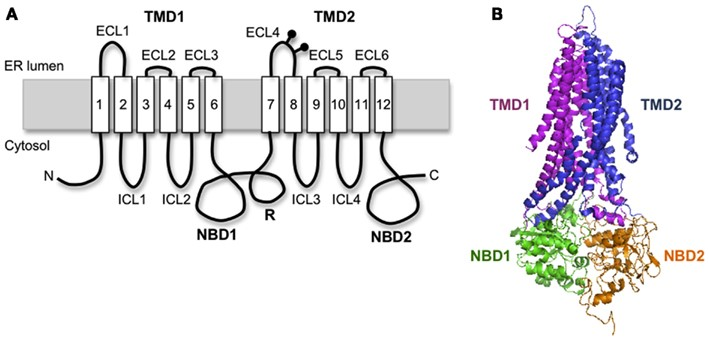
\includegraphics[scale=2]{gfx/CFTR.jpg} 
\captionsetup{type=figure}
\captionof{figure}{Structure CFTR}
       \label{cftr}
\end{center}

		\section{Fonction}
Le rôle de la protéine CFTR est toujours sujet à spéculations, mais il est maintenant admis que CFTR est une protéine multifonctionnelle. Une de ces fonctions principale est d’être un canal chlorure indépendant du voltage et du temps, mais dépendant de l’AMPc (régulation via PKA et PKC par phosphorylation), utilisant l’hydrolyse de l’ATP comme énergie et ayant une faible conductance (Anderson, Berger, et al. 1991; Anderson, Gregory, et al. 1991)\cite{anderson_nucleoside_1991}\cite{anderson_demonstration_1991}. CFTR forme un canal anionique permettant la diffusion passive des ions chlorure, le mécanisme de sélectivité de charge est lié aux segments transmembranaires TM1 et TM6. (Dawson, Smith, and Mansoura 1999; Linsdell 2006)\cite{dawson_cftr:_1999}\cite{linsdell_mechanism_2006}. La séquence de sélectivité du canal CFTR est : Br- (Bromure)>Cl- (Chlorure)>I- (Iodure)>F-(Fluorure). Cette perméabilité du Cl- plus importante que celle de l’I- différencie CFTR des autres canaux chlorure pour qui cette séquence est inversée(Sheppard and Welsh 1999)\cite{sheppard_structure_1999}. Possédant une sélectivité plus grande pour les anions plutôt que pour les cations monovalents, CFTR semble aussi perméable au tripeptide glutathion (GSH) qui est l’antioxydant le plus abondamment retrouvé dans les poumons (Kogan et al. 2003)\cite{kogan_cftr_2003}.
CFTR est aussi une protéine régulatrice de courant chlorure, elle possède donc aussi des propriétés de régulation de la conductance membranaire. Elle a été montrée comme étant un acteur majeur de la régulation du canal ORCC (Outwardly Rectifying Chloride Channel) de par sa présence fonctionnelle indispensable à l'activation du canal ORCC par les PKA(Devidas and Guggino 1997)\cite{devidas_cftr:_1997}. CFTR est aussi régulatrice d’autres protéines comme le canal sodique ENaC (Epithelial Na+ Channel), elle le régule négativement(Devidas and Guggino 1997)\cite{devidas_cftr:_1997}. Son absence entraine une hyper-absorption de Na+ ce qui a pour conséquence la déshydratation du mucus (Letz and Korbmacher 1997)\cite{letz_camp_1997}. Pour l’inhibition des canaux potassiques ROMK (Renal Outer Medullary Potassium channel) par l’ATP cytosolique, CFTR est nécessaire (Ruknudin et al. 1998)\cite{ruknudin_novel_1998}. Enfin une régulation positive des aquaporines par CFTR participe à l’hydratation du mucus (Schwiebert et al. 1999; Schreiber et al. 2000) \cite{schwiebert_cftr_1999}\cite{schreiber_aquaporin_2000}
En conclusion la fonction de CFTR est de réguler le transport des ions et les mouvements d’eau au travers de la barrière épithéliale des cellules qui produisent du mucus, de la sueur ou de la salive. Sans altération CFTR fonctionne comme un canal à travers la membrane et transporte les ions chlorure négativement chargé en dehors de la cellule afin d’aider au contrôle des mouvements d’eau dans les tissus, élément nécessaire pour la production d’un fin mucus qui va protéger les voies aériennes, le système digestif et reproducteur, ainsi que d’autre organes et tissues. 

		\section{Mutation CFTR}
Jusqu’à présent plus de 1900 mutations ont été identifié. Dans l’ensemble des mutations recensées, les plus communes sont les mutations faux-sens (48.7\%), suivi par des modifications du cadre de lecture causé par une petite insertion ou délétion (19.5\%), puis des mutations altérant des codons essentiels pour l’épissage (15.7\%) et enfin des mutations non-sens (12.9\%). En fonction du dysfonctionnement moléculaire observé sur CFTR ces mutations ont été réparties dans différentes catégories, on dénombre six classes (Kerem 2006)\cite{kerem_mutation_2006}. Alors que les trois dernières classes sont associées à un phénotype mucoviscidosique modéré, les trois premières sont beaucoup plus sévères (Figure \ref{mutation}):
\begin{itemize}
\item Mutations de classe I conduisent à un défaut de production de la protéine CFTR qui est complètement absente, ce sont les deuxièmes mutations les plus communes.
\item Mutations de classe II conduisent à un défaut de maturation de CFTR, ce qui a pour conséquence d’affecter l’adressage de la protéine dans le réticulum endoplasmique et l’appareil de golgi. Ceci est dû à une mauvaise glycosylation et repliement de la protéine ne formant pas une structure tertiaire appropriée et qui finit donc par être ciblé par la dégradation au lieu d’être envoyée à la membrane apicale. Ce sont les mutations les plus communes on y retrouve la mutation $\Delta508$F qui représente 70\% des mutations observé chez les patients atteint de mucoviscidose. 
\item Mutations de classe III et IV, la protéine CFTR est normalement traduite et normalement adressé à la membrane apicale, mais il manque une complète activité de son canal ionique. Dans le cas des mutations de classe III on a un défaut de régulation de CFTR dû à une diminution de la probabilité d’ouverture du canal. Pour les mutations de classe IV on a une altération de la conduction du canal, les mutations peuvent induire des modifications de sa sélectivité ainsi qu’une diminution du flux ionique. 
\item Mutations de classe V résulte en une altération de stabilité de l’ARN messager conduisant à un nombre diminué de copie de CFTR et donc à un trafique appauvrie à la membrane plasmique. 
\item Mutations de classe VI sont à l’origine d’une altération de stabilité de la protéine mature, on a une accélération du turnover de la protéine CFTR à la surface de la cellule et donc à une diminution de sa quantité.
\end{itemize}

\begin{center}
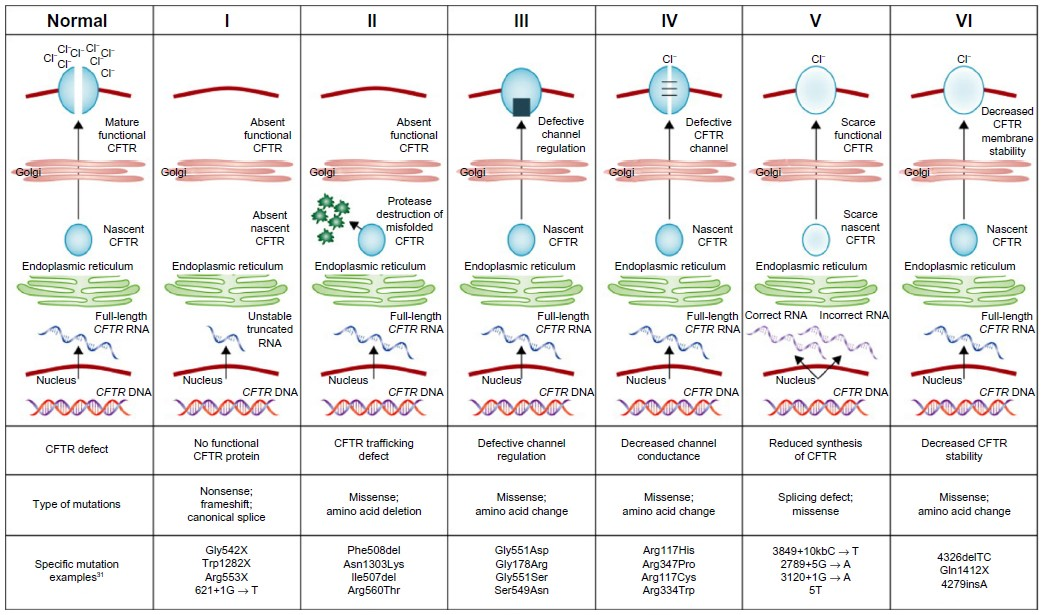
\includegraphics[scale=0.4]{gfx/mutation.jpg} 
\captionsetup{type=figure}
\captionof{figure}{Classes de mutation de CFTR}
       \label{mutation}
\end{center}
 
Ces mutations ont de multiples conséquences principalement un défaut de transport d’ion et de mouvement d’eau à l’intérieur et l’extérieur de la cellule et qui a pour conséquence une production d’un mucus épais par les organes à tissus épithéliaux sécréteurs. Ce mucus va notamment avoir pour effet d’obstruer les voies respiratoires et les glandes, menant à des signes et symptômes caractéristiques de la mucoviscidose notamment une inflammation chronique qui reste la cause principale de mortalité et morbidité

%------------------------------------------------

% \subsection{Subsection Title}

% Content